\documentclass{article}
\usepackage{tikz}
\usetikzlibrary{arrows.meta,positioning,calc,shapes.geometric}
\pagestyle{empty}
\begin{document}
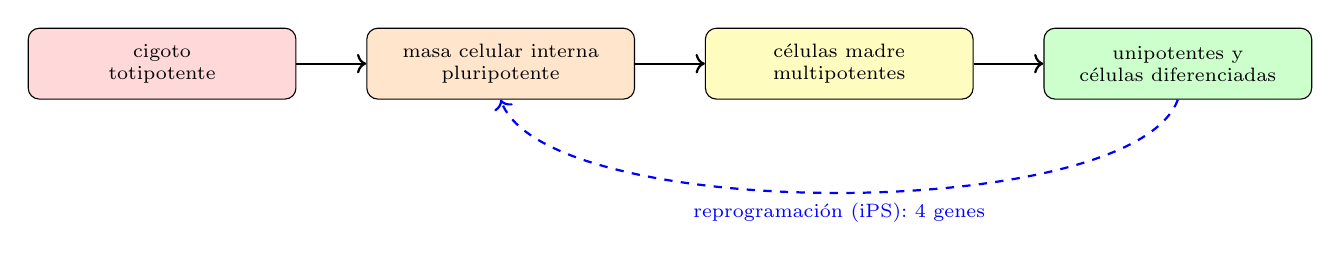
\begin{tikzpicture}
\tikzset{every node/.append style={align=center}}

\node[draw, rounded corners, fill=red!15, minimum width=3.4cm, minimum height=0.9cm, align=center, font=\scriptsize] (z) at (0,0) {cigoto\\ totipotente};
\node[draw, rounded corners, fill=orange!20, minimum width=3.4cm, minimum height=0.9cm, align=center, font=\scriptsize] (b) at (4.3,0) {masa celular interna\\ pluripotente};
\node[draw, rounded corners, fill=yellow!25, minimum width=3.4cm, minimum height=0.9cm, align=center, font=\scriptsize] (m) at (8.6,0) {células madre\\ multipotentes};
\node[draw, rounded corners, fill=green!20, minimum width=3.4cm, minimum height=0.9cm, align=center, font=\scriptsize] (u) at (12.9,0) {unipotentes y\\ células diferenciadas};
\draw[->, thick] (z) -- (b); \draw[->, thick] (b) -- (m); \draw[->, thick] (m) -- (u);
\draw[->, thick, dashed, blue] (u.south) to[out=-110, in=-70, looseness=0.5] node[below, font=\scriptsize] {reprogramación (iPS): 4 genes} (b.south);

\end{tikzpicture}
\end{document}
